\documentclass[10pt,aspectratio=169]{beamer}

\usetheme{Madrid}
\usefonttheme{professionalfonts}
\setbeamertemplate{navigation symbols}{}
\setbeamertemplate{caption}[numbered]
\setbeamerfont{frametitle}{series=\bfseries,size=\large}
\setbeamerfont{title}{series=\bfseries,size=\Large}

\usepackage[T1]{fontenc}
\usepackage{lmodern}
\usepackage{microtype}
\usepackage{amsmath,amssymb}
\usepackage{booktabs}
\usepackage{tabularx}
\usepackage{array}
\usepackage{graphicx}
\usepackage{xcolor}
\usepackage{tikz}
\usetikzlibrary{positioning,arrows.meta}
\usepackage{url}

\graphicspath{{results/presentation/}{results/}{./}}

\definecolor{DeepNavy}{HTML}{0B1F3A}
\definecolor{Photon}{HTML}{007C89}
\definecolor{Muted}{HTML}{5B6472}
\definecolor{Mist}{HTML}{EEF6F6}
\definecolor{Amber}{HTML}{D97706}

\setbeamercolor{normal text}{fg=black,bg=white}
\setbeamercolor{structure}{fg=Photon}
\setbeamercolor{title}{fg=white,bg=DeepNavy}
\setbeamercolor{frametitle}{fg=white,bg=DeepNavy}
\setbeamercolor{block title}{fg=white,bg=Photon}
\setbeamercolor{block body}{fg=black,bg=Mist}
\setbeamercolor{footline}{fg=white,bg=DeepNavy}

\newcolumntype{Y}{>{\raggedright\arraybackslash}X}
\newcommand{\pjbit}{pJ/bit}
\newcommand{\tbps}{Tb/s}
\newenvironment{tightitemize}{\begin{itemize}\setlength{\itemsep}{4pt}\setlength{\parskip}{0pt}}{\end{itemize}}
\newenvironment{tightenumerate}{\begin{enumerate}\setlength{\itemsep}{4pt}\setlength{\parskip}{0pt}}{\end{enumerate}}

\title[Photonic Interconnects for TPU LLMs]{Topology-Aware Mapping for Photonic Interconnects in TPU-Class LLM Accelerators}
\subtitle{6.5930 Project 12: Evaluate a New Technology}
\author[Sitaraman \& Surdi]{Pranav Sitaraman \and Simone Surdi}
\institute[MIT 6.5930]{Hardware Architectures for Deep Learning}
\date{Spring 2026}

\begin{document}

\begin{frame}
  \titlepage
  \vspace{-0.4em}
  \begin{center}
    {\small Emerging technology study: Lightmatter Passage photonic interconnect}
  \end{center}
\end{frame}

\begin{frame}{The One-Slide Thesis}
  \begin{columns}[T,onlytextwidth]
    \begin{column}{0.32\textwidth}
      \begin{block}{$42.4\times$}
      Best modeled inference latency speedup. Gemma~4 26B mixture-of-experts on a 9216-chip pod.
      \end{block}
    \end{column}
    \begin{column}{0.32\textwidth}
      \begin{block}{$0$ of $24$}
      Local mapping signatures that change under the photonic swap on the 64-chip torus.
      \end{block}
    \end{column}
    \begin{column}{0.32\textwidth}
      \begin{block}{$5$ of $16$}
      Distributed schedule choices that change once multicast and pooled remote memory become cheap.
      \end{block}
    \end{column}
  \end{columns}
  \vspace{0.6em}
  \begin{block}{The claim}
  Photonic interconnect is not just a lower-\pjbit{} wire. Where it really earns its keep is enabling a different distributed schedule above the local mapping: multicast cache fill, remote pooled-HBM streaming, and a flatter, switched fabric in place of the long electrical hops.
  \end{block}
\end{frame}

\begin{frame}{Why This Belongs in a TPU/LLM Conversation}
  \begin{columns}[T,onlytextwidth]
    \begin{column}{0.55\textwidth}
      \begin{tightitemize}
        \item TPU7x/Ironwood is publicly documented at 9216 chips per pod, 192~GiB of HBM per chip, and 1200~GB/s of bidirectional inter-chip bandwidth per chip.
        \item Decode caches, expert tokens, gradients, and shared weights are all moved across chips during normal training and inference.
        \item Production software already treats the pod as a sharded device mesh: GSPMD-style annotations choose where data lives and the compiler inserts the matching collectives.
      \end{tightitemize}
    \end{column}
    \begin{column}{0.42\textwidth}
      \begin{block}{The question we asked}
      If a future TPU pod were wired with Lightmatter-style photonics, would the mapper just see cheaper bits, or would the optimal placement and schedule above the mapper actually change?
      \end{block}
    \end{column}
  \end{columns}
\end{frame}

\begin{frame}{The Experiment Spine}
  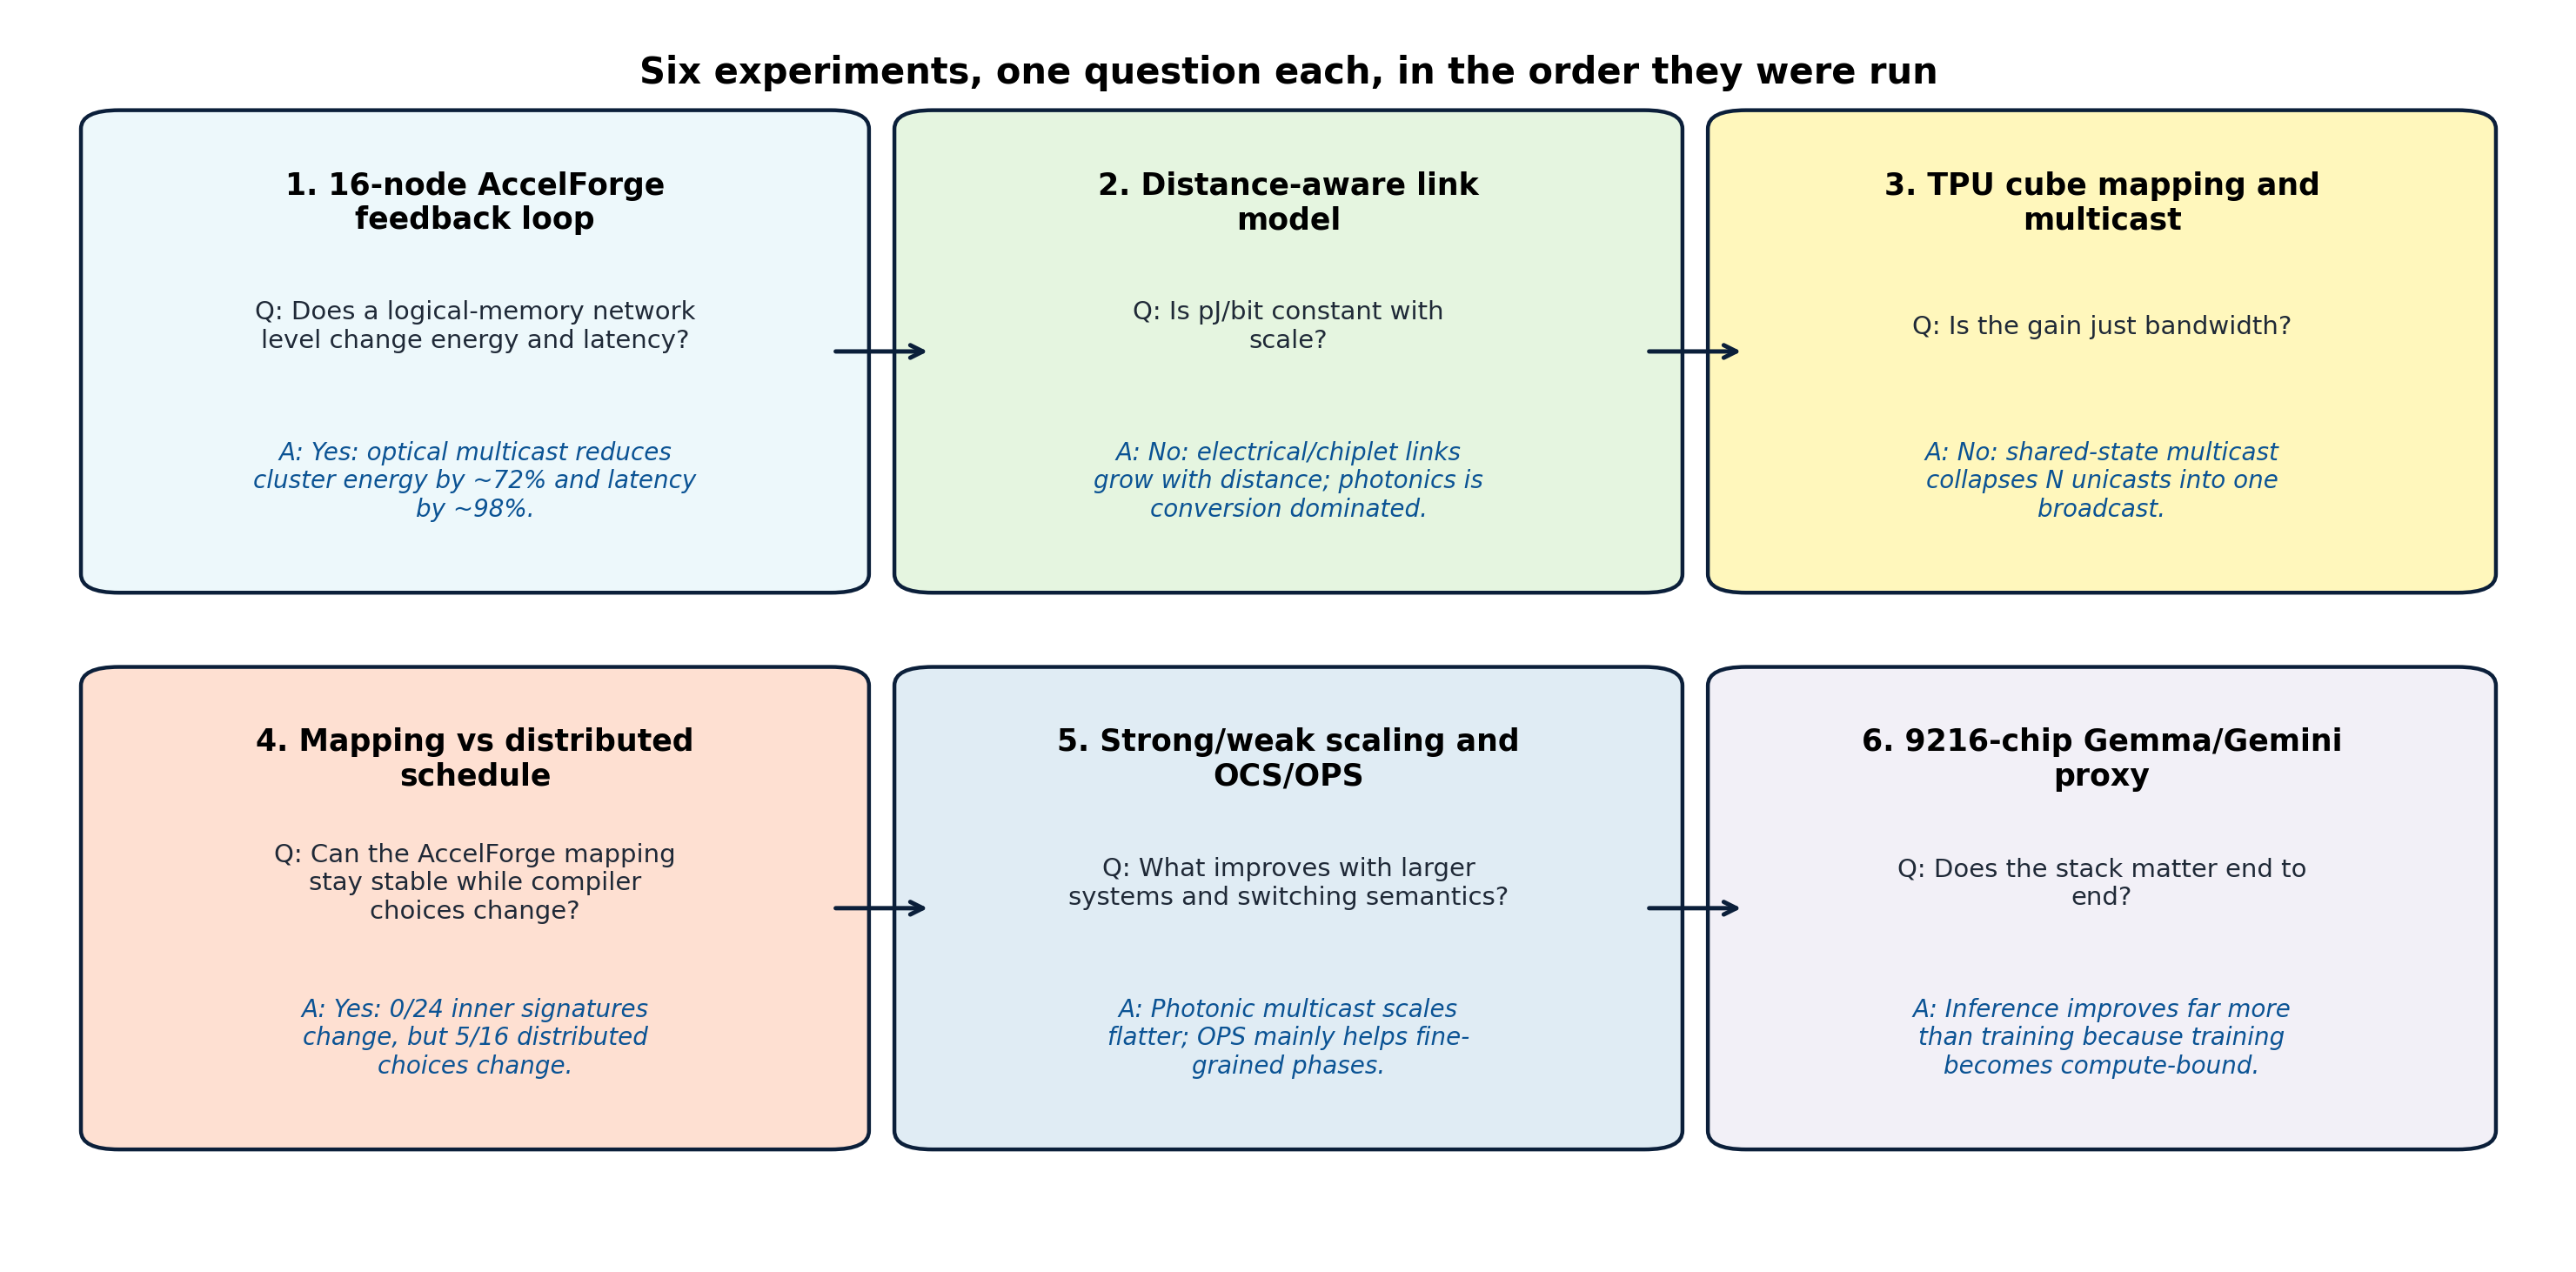
\includegraphics[width=\linewidth,height=0.78\textheight,keepaspectratio]{01_evidence_chain.png}
\end{frame}

\begin{frame}{What ``Mapping'' Means in This Study}
  \begin{columns}[T,onlytextwidth]
    \begin{column}{0.55\textwidth}
      \begin{tightenumerate}
        \item \textbf{Workload:} a parameterized GEMM einsum that stands in for a particular LLM stage.
        \item \textbf{Architecture:} the per-chip memory hierarchy plus a logical cluster-memory level above it.
        \item \textbf{Inner mapping:} the loop order, tile shape, and tensor residency that the mapper picks locally.
        \item \textbf{Distributed schedule:} the compiler-visible decision about whether traffic is point-to-point, fetched from a remote pool, or multicast from a shared source.
      \end{tightenumerate}
    \end{column}
    \begin{column}{0.42\textwidth}
      \begin{block}{Why the split matters}
      The inner mapping can stay identical while the distributed schedule above it changes, and that is exactly what we see in our experiments. Reporting them together would have hidden the actual mechanism.
      \end{block}
    \end{column}
  \end{columns}
\end{frame}

\begin{frame}{Network Cost Folded Back Into Memory}
  \begin{columns}[T,onlytextwidth]
    \begin{column}{0.48\textwidth}
      \[
      E_{\text{net}}=B\bigl(e_c+h\,\ell(N)\,e_{tx}\bigr)
      \]
      \[
      T_{\text{net}}=\frac{B}{BW/C(N)}+h\,t_r+h\,\ell(N)\,t_p+t_s
      \]
      \begin{tightitemize}
        \item $B$: bits transferred, taken from mapper action counts.
        \item $h$: average hop count for the topology.
        \item $\ell(N)$: average physical path distance.
        \item $C(N)$: contention factor under $N$ active nodes.
        \item $t_s$: optical-switching reconfiguration term.
      \end{tightitemize}
    \end{column}
    \begin{column}{0.49\textwidth}
      \begin{block}{Iterative loop}
      Mapper $\rightarrow$ logical-memory traffic $\rightarrow$ topology cost $\rightarrow$ updated logical-memory energy and latency $\rightarrow$ mapper rerun, until the per-bit numbers stabilize.
      \end{block}
      \begin{block}{The multicast rule}
      Electrical and chiplet baselines pay every receiver. Multicast-capable photonics pays the unique payload exactly once.
      \end{block}
    \end{column}
  \end{columns}
\end{frame}

\begin{frame}{Assumptions Kept Visible}
  \scriptsize
  \begin{tabularx}{\linewidth}{lYY}
  \toprule
  Item & Value & Role \\
  \midrule
  Ironwood pod & 9216 chips; 192~GiB HBM/chip; 1200~GB/s ICI/chip & Full-system baseline \\
  M1000 photonic & 57.3~\tbps{} one-way, 2.3~\pjbit{} including laser & Main photonic fabric \\
  EVK100 photonic & 3.2~\tbps{} class, 1.9--3.2~\pjbit{} & Conservative and optimistic sensitivity points \\
  Electrical link & 0.2~\pjbit{} conversion + 1.96~\pjbit{}/mm transmission & Distance-sensitive baseline \\
  Chiplet baseline & 3.5~\tbps{}, 6~\pjbit{}/hop & Strong non-optical comparison \\
  Compiler layer & SPMD collectives, remote pooled HBM, replicated cache, photonic multicast & GSPMD-style schedule choices \\
  \bottomrule
  \end{tabularx}
  \vspace{0.6em}
  \footnotesize\textit{The compute side, the per-chip memory hierarchy, and the HBM cost are held fixed across every comparison. Only interconnect, topology, multicast, and the distributed schedule change.}
\end{frame}

\begin{frame}{Result 1: Distance Reshapes the Scaling Law}
  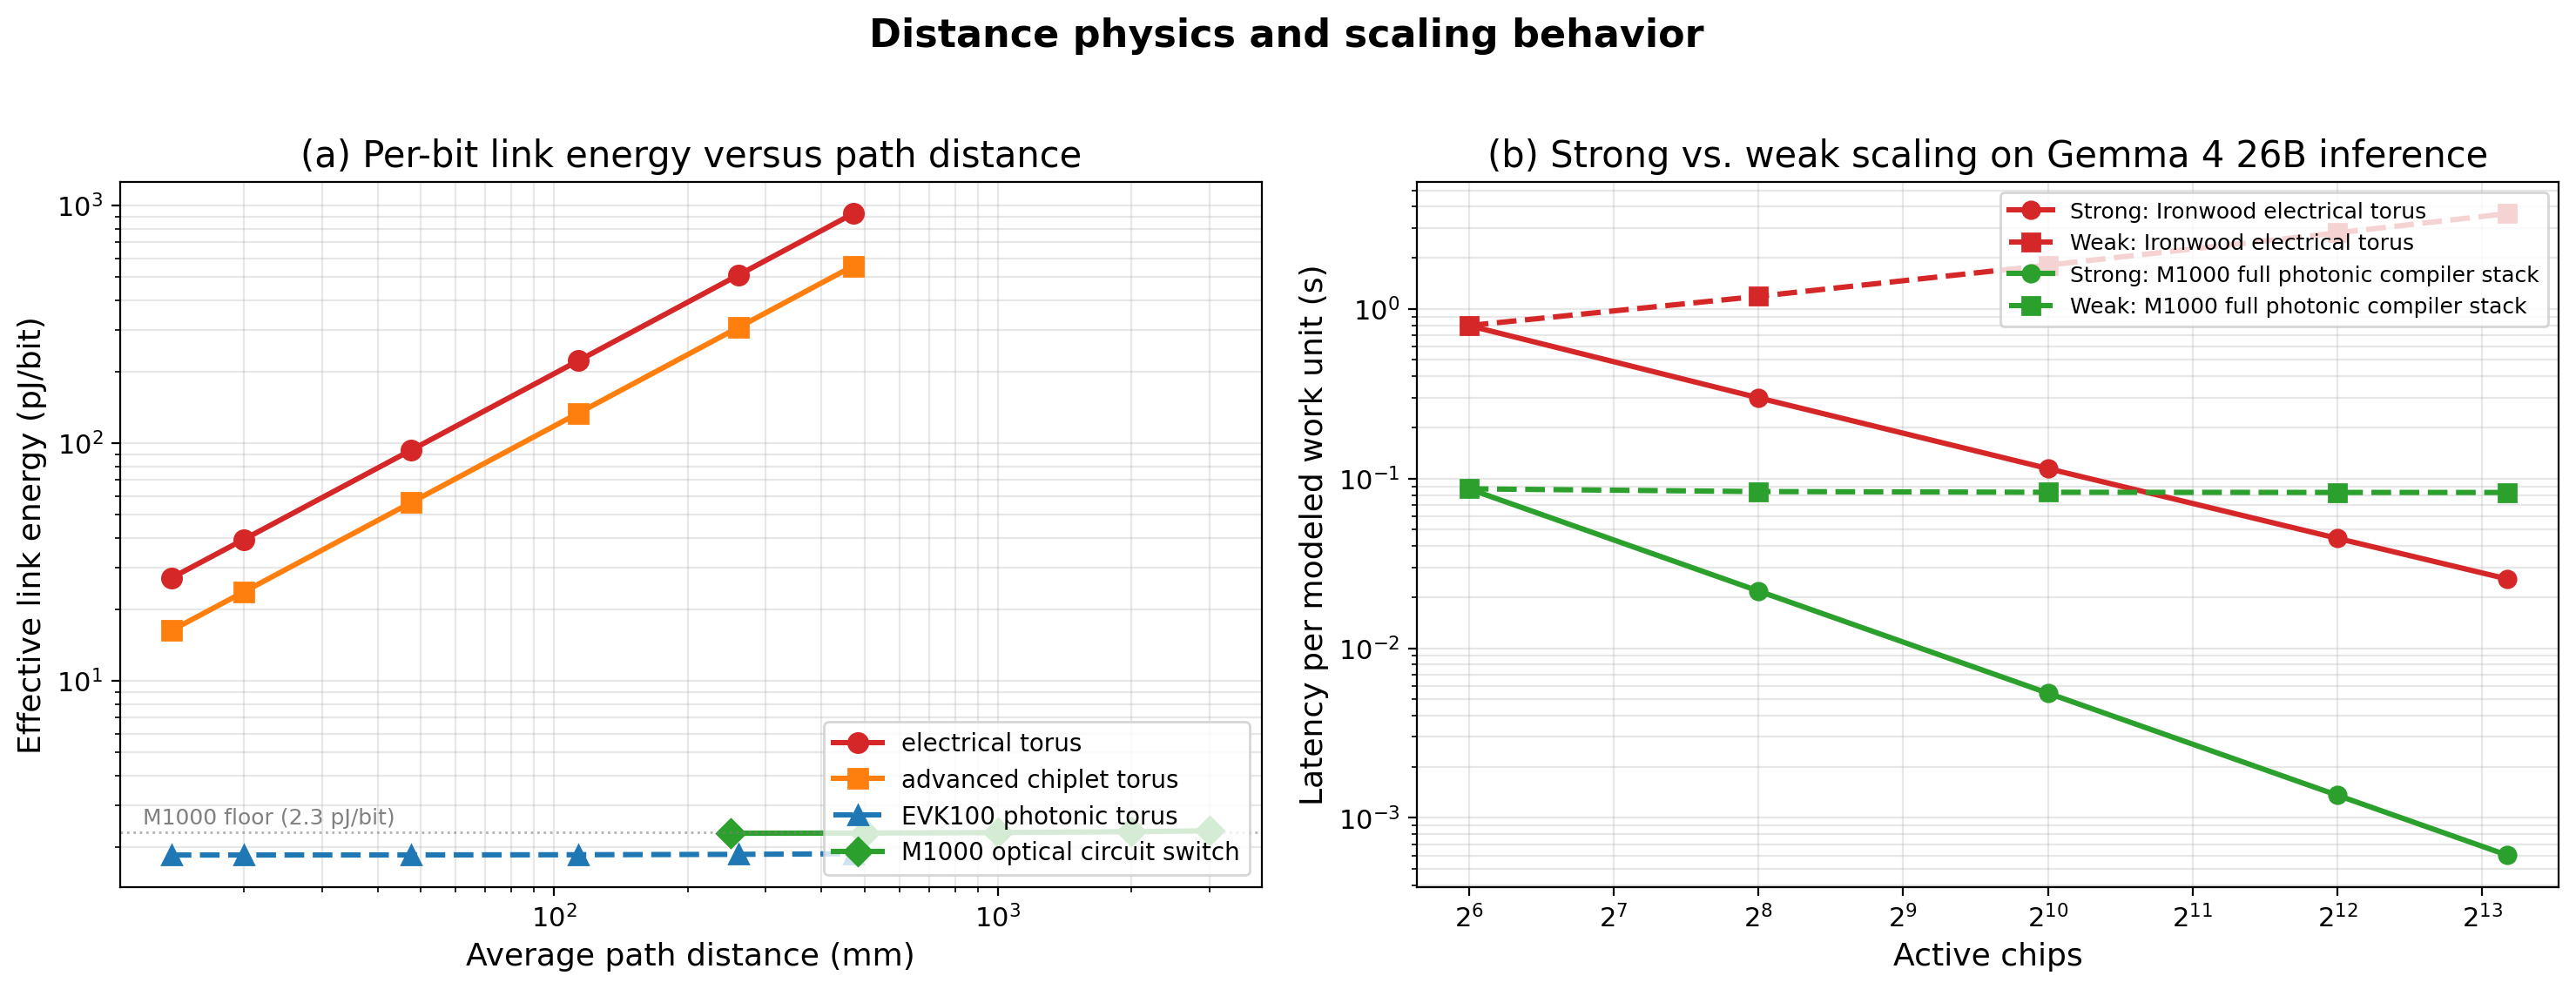
\includegraphics[width=\linewidth,height=0.78\textheight,keepaspectratio]{02_distance_and_scaling.png}
\end{frame}

\begin{frame}{Reading Result 1}
  \begin{tightitemize}
    \item Electrical and chiplet links are good at very short reach but accumulate transmission energy with distance.
    \item Photonic links pay their conversion energy once and stay nearly flat, so the curves cross over before pod scale.
    \item Strong scaling and weak scaling are kept separate to avoid conflating ``faster on fixed work'' with ``more aggregate throughput.''
    \item This is also the reason a constant-\pjbit{} comparison would have been misleading: it would have hidden which side of the crossover each topology lives on.
  \end{tightitemize}
\end{frame}

\begin{frame}{Result 2: The Local Mapping Does Not Move}
  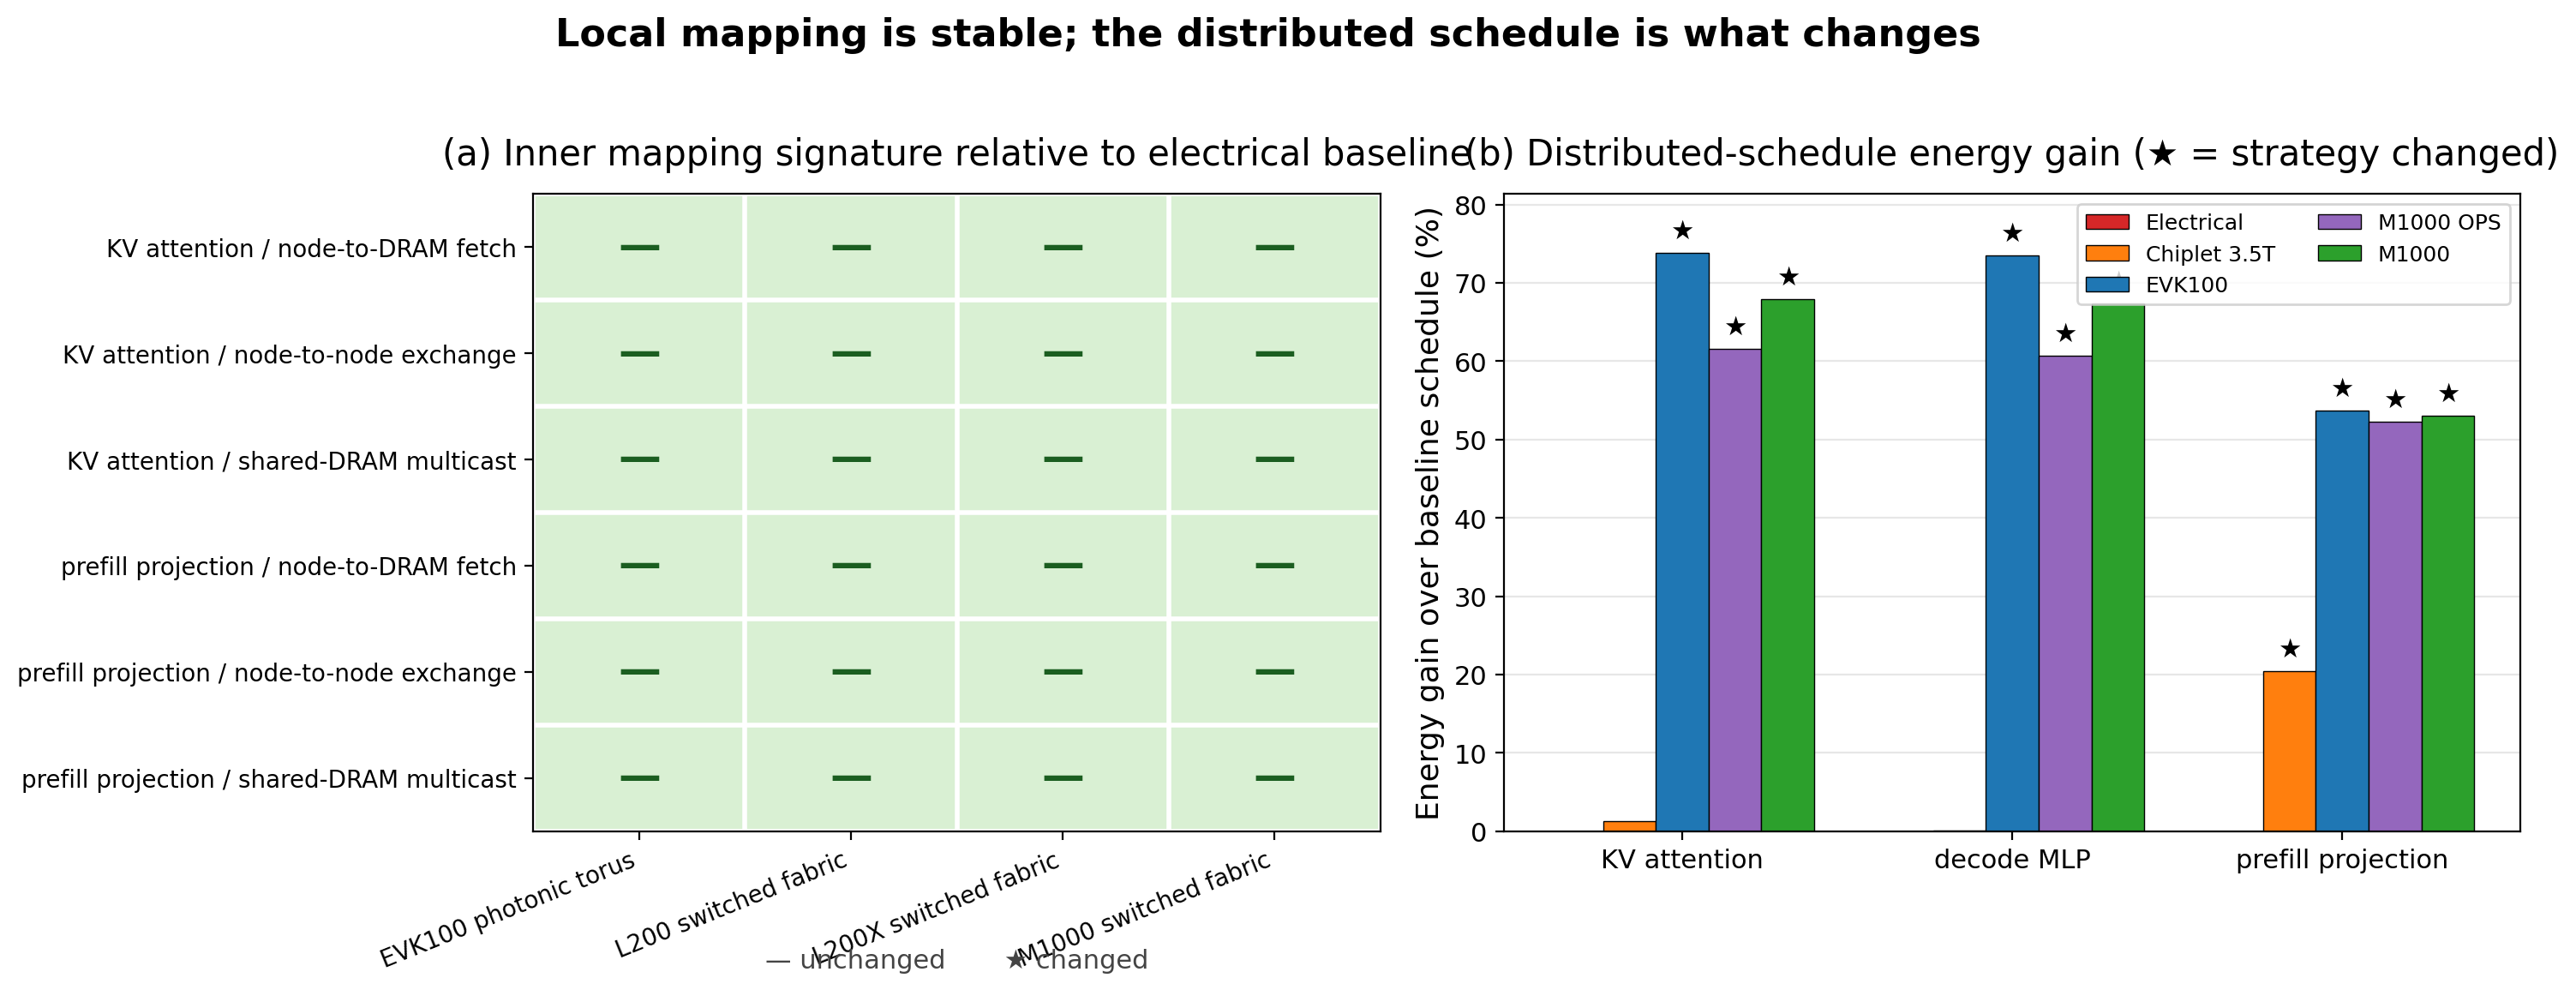
\includegraphics[width=\linewidth,height=0.78\textheight,keepaspectratio]{03_mapping_and_schedule.png}
\end{frame}

\begin{frame}{Reading Result 2}
  \begin{tightitemize}
    \item Across all photonic torus and switched-fabric variants on the 64-chip cube, the local mapping signature is the same as the electrical baseline. Every cell on the left is unchanged.
    \item One layer up, the picture is the opposite. Photonic technologies prefer remote pooled-HBM streaming for decode and KV attention, and they prefer shared-DRAM multicast for prefill projection.
    \item The electrical and chiplet baselines see almost no benefit from those alternative schedules, because the corresponding traffic is too expensive on those links.
    \item This is the cleanest evidence we have that the photonic gain is mostly above the mapper, in compiler-visible territory.
  \end{tightitemize}
\end{frame}

\begin{frame}{Result 3: Multicast and the Strong Chiplet Baseline}
  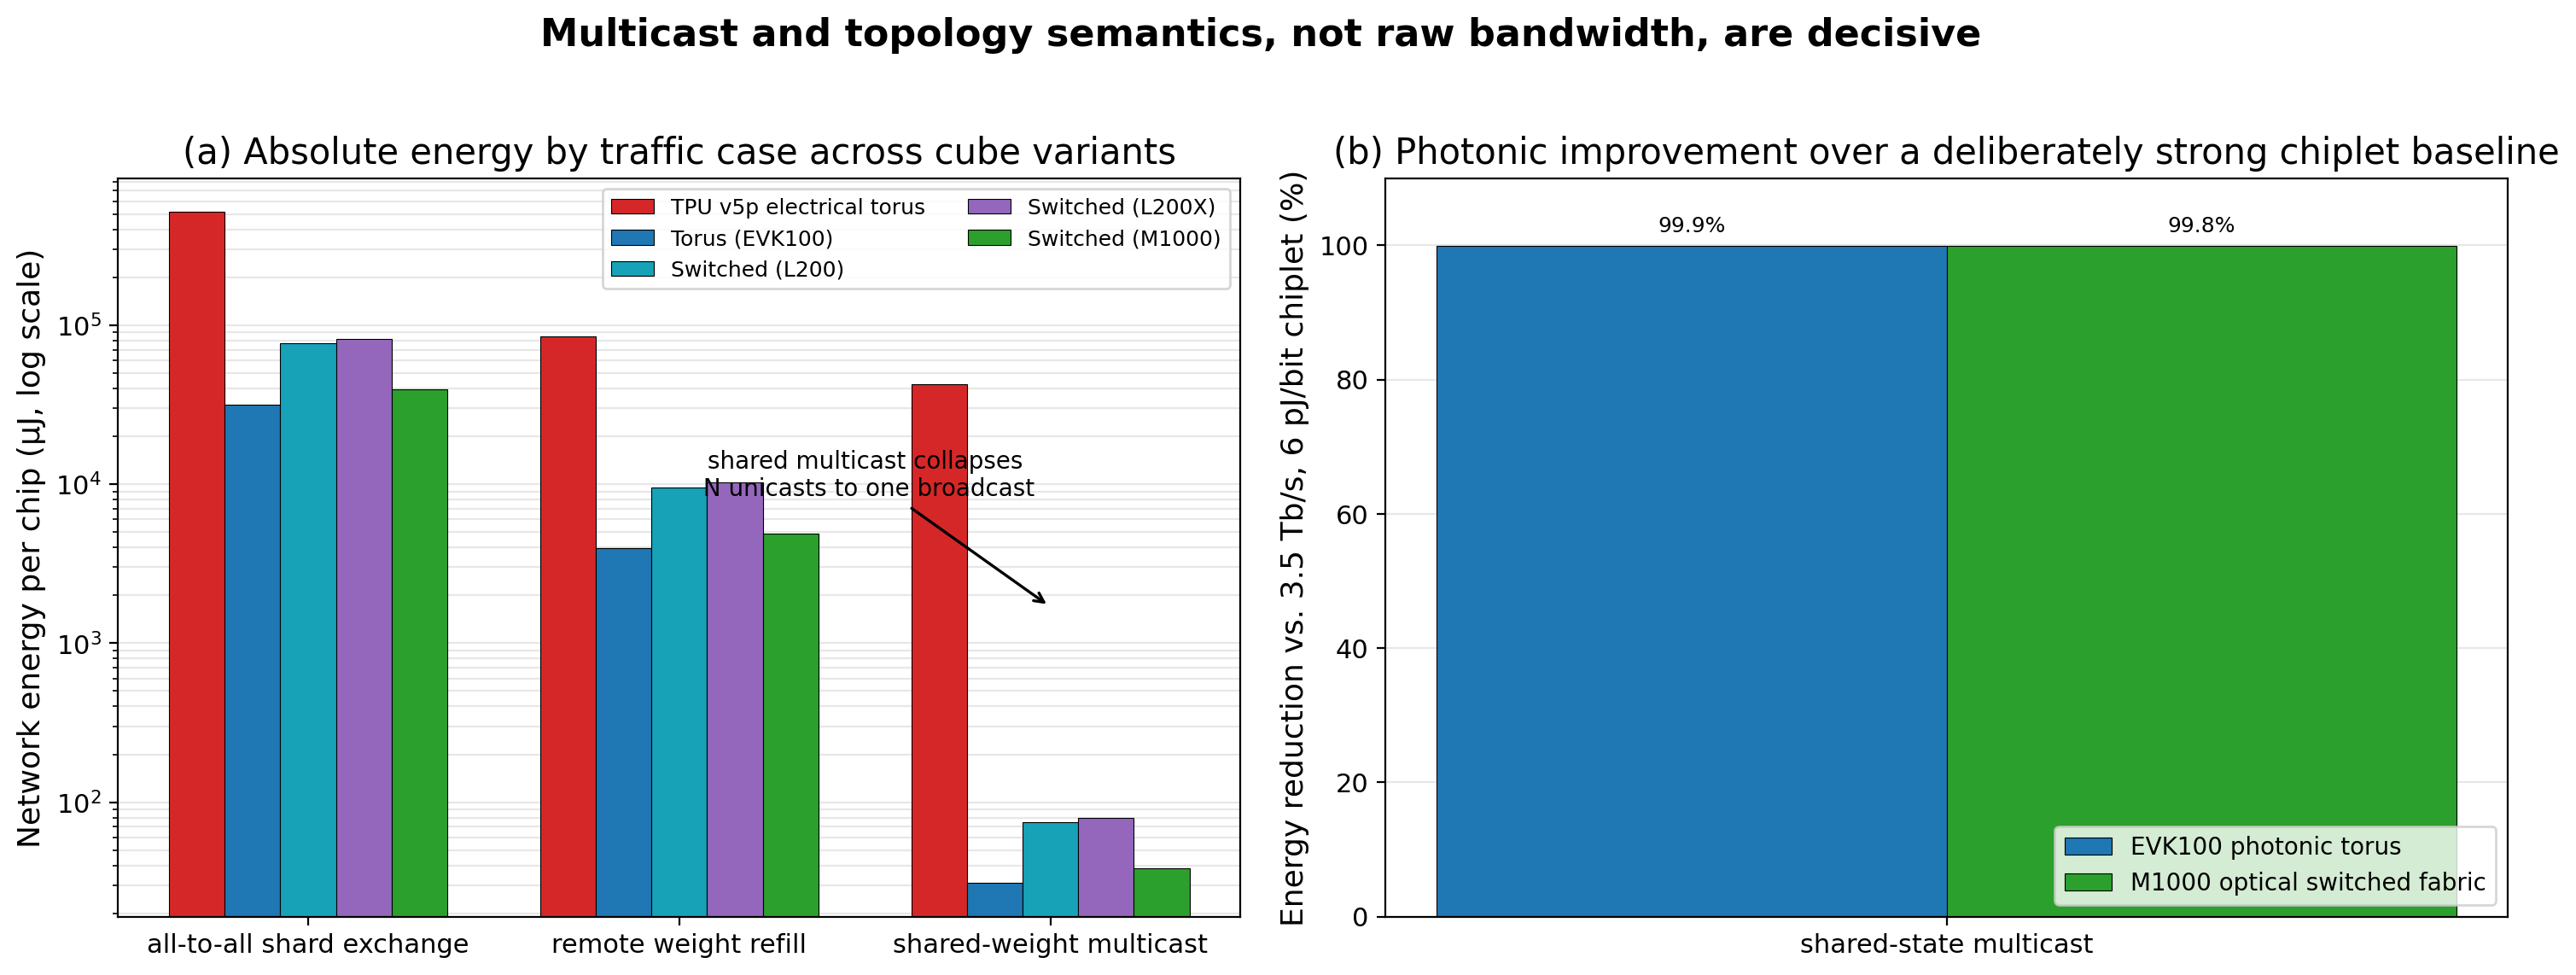
\includegraphics[width=\linewidth,height=0.78\textheight,keepaspectratio]{04_multicast_and_chiplet.png}
\end{frame}

\begin{frame}{Reading Result 3}
  \begin{tightitemize}
    \item The chiplet baseline is deliberately not weak: 3.5~\tbps{} and 6~\pjbit{}/hop, similar to advanced packaging targets.
    \item The shard-exchange and weight-refill cases are roughly an order of magnitude below the electrical torus across photonic variants. The shared-multicast case is closer to four orders of magnitude below it.
    \item The reason is structural rather than bandwidth-driven: shared multicast collapses $N$ unicast deliveries into one logical broadcast. That is a topology-semantics effect, not a wire effect.
    \item Workloads that cannot exercise that pattern see far smaller gains. We keep both kinds of cases in view rather than reporting only the favorable ones.
  \end{tightitemize}
\end{frame}

\begin{frame}{Result 4: 16-Node Validation Heatmap}
  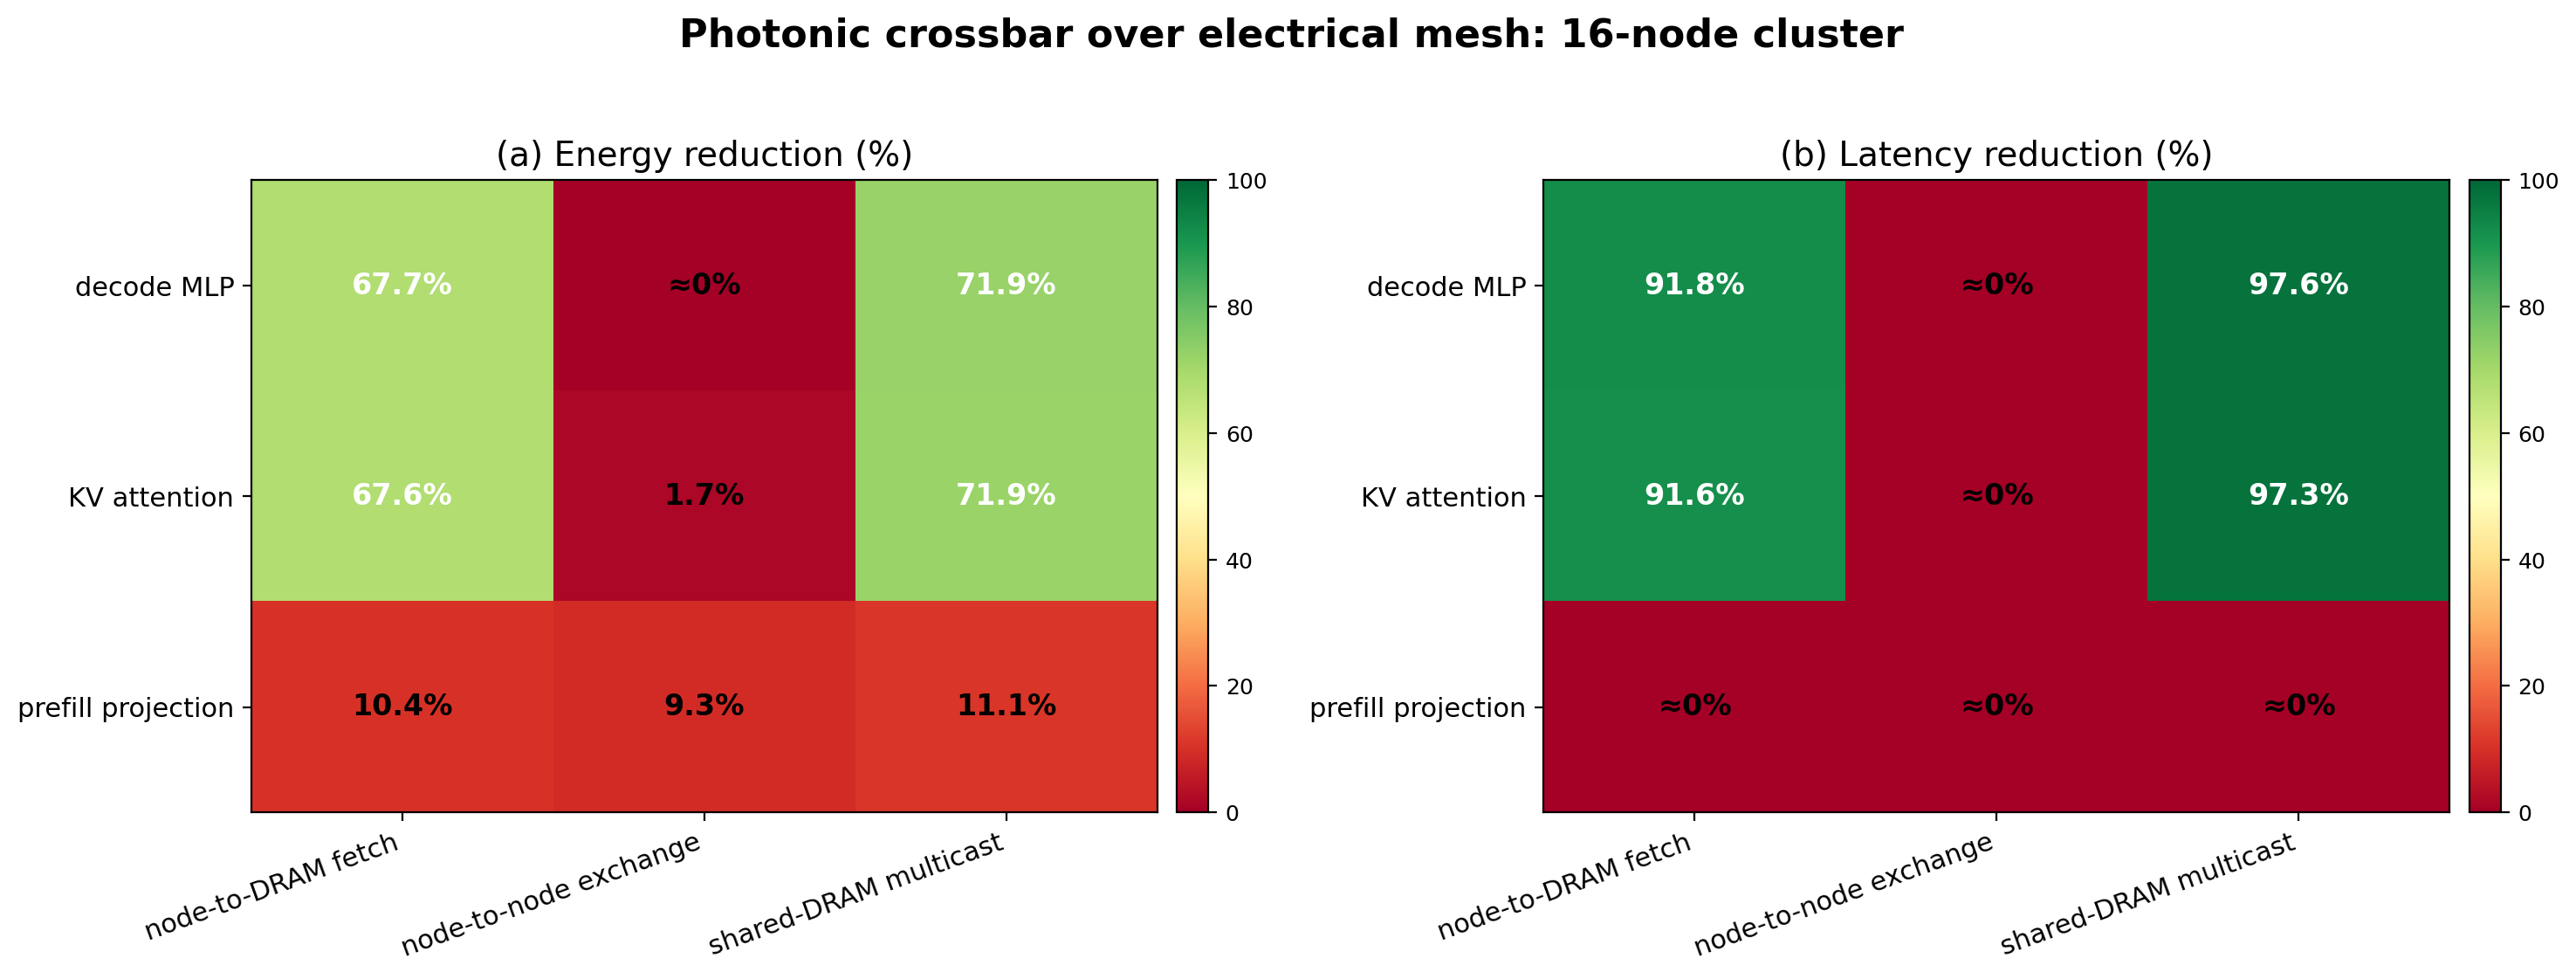
\includegraphics[width=\linewidth,height=0.78\textheight,keepaspectratio]{07_cluster_workload_heatmap.png}
\end{frame}

\begin{frame}{Result 5: End-to-End Pod Impact}
  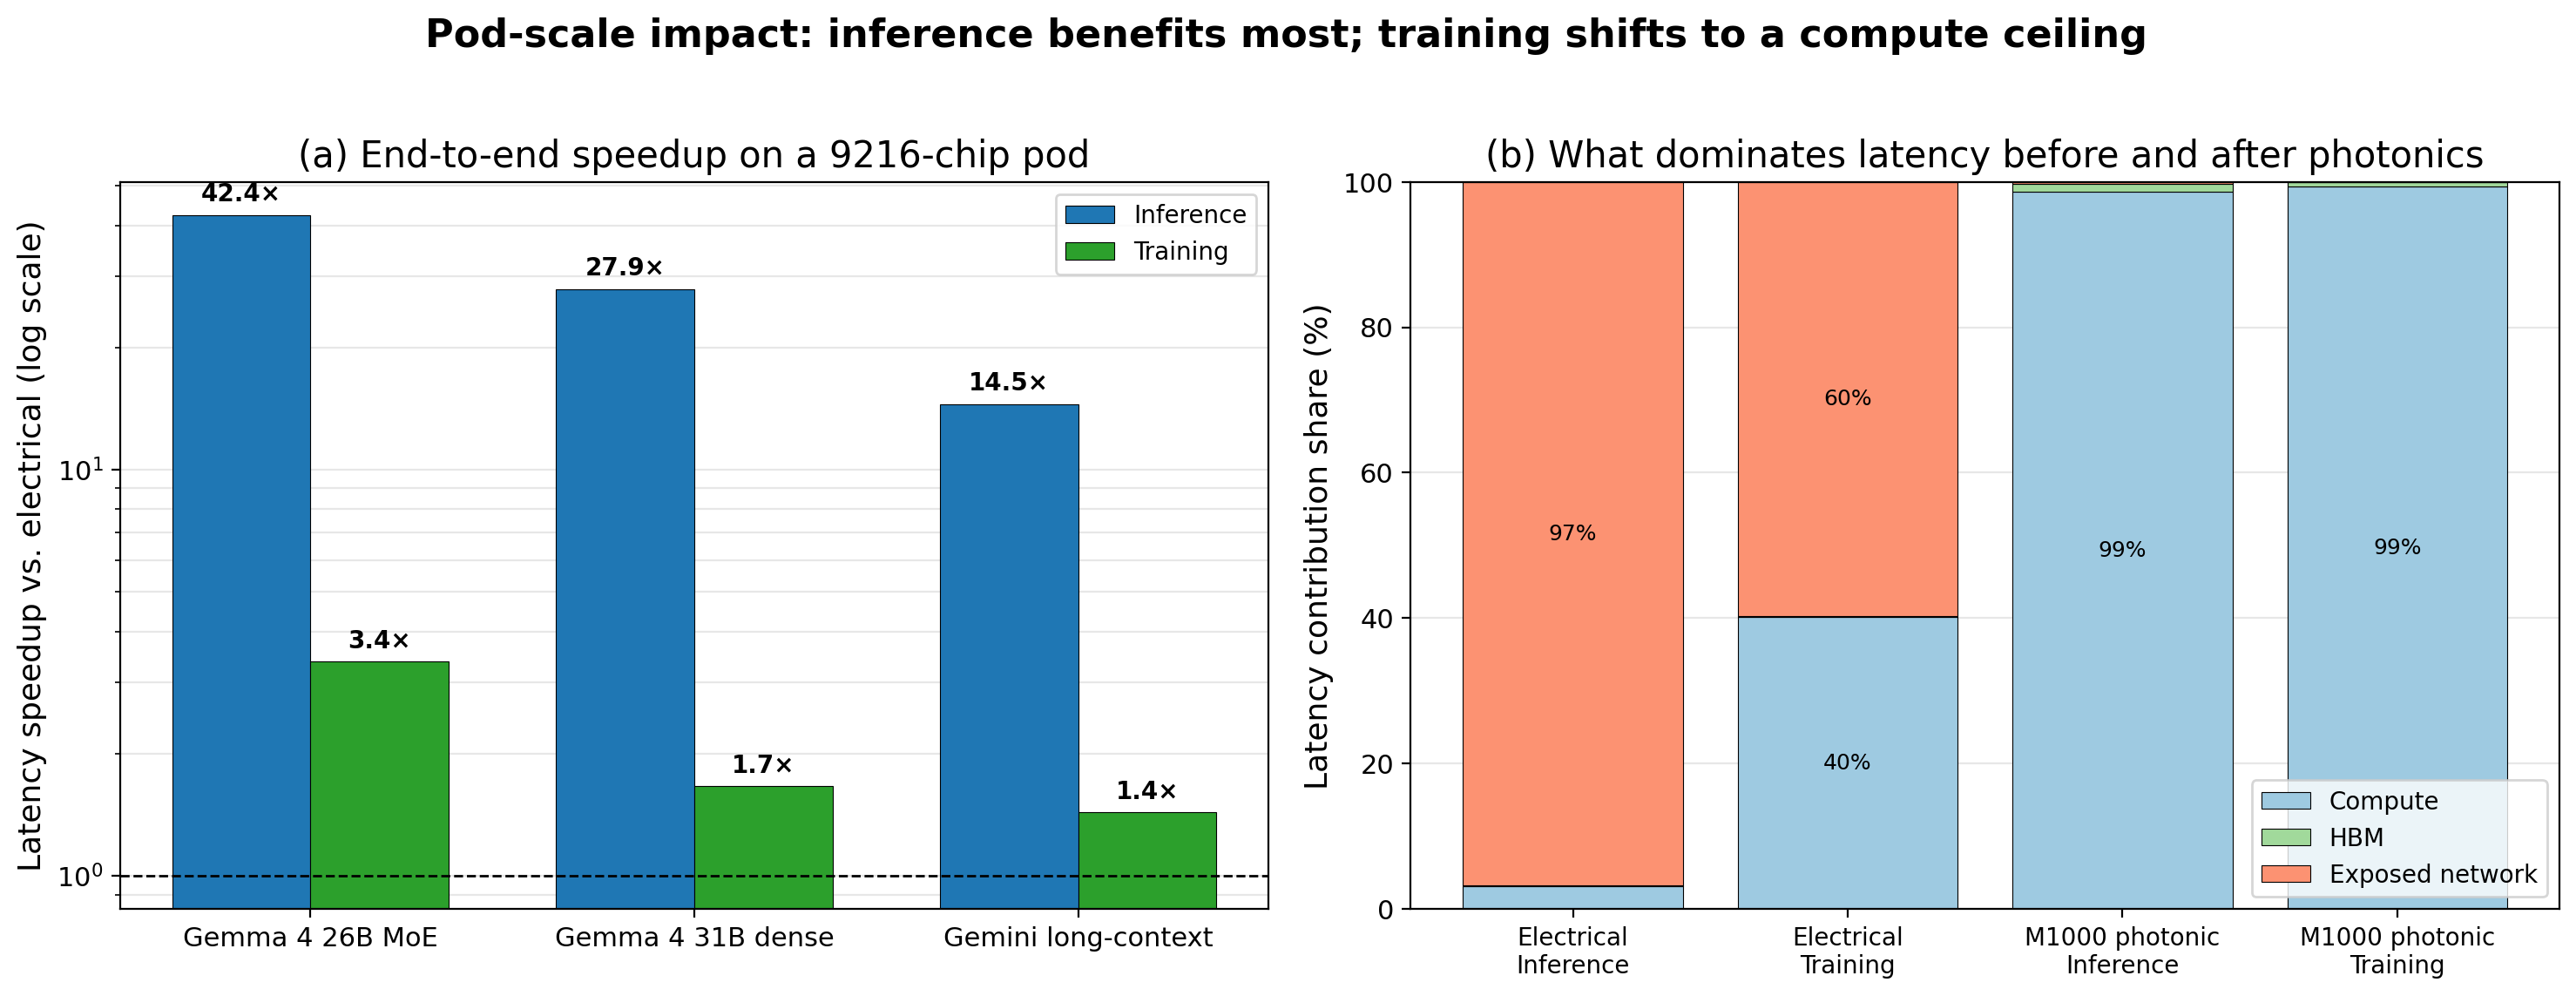
\includegraphics[width=\linewidth,height=0.78\textheight,keepaspectratio]{05_superpod_end_to_end.png}
\end{frame}

\begin{frame}{Reading Result 5}
  \begin{tightitemize}
    \item Inference latency on the Gemma~4 26B mixture-of-experts proxy improves by roughly $42\times$. The long-context Gemini proxy improves by roughly $15\times$.
    \item Training improvements are far smaller---about $3.4\times$ and $1.4\times$ respectively---because once communication shrinks, what is left is matrix-multiply compute.
    \item The right panel makes the regime change concrete. Electrical inference is overwhelmingly network-bound. Photonic inference is overwhelmingly compute-bound. That is the textbook signature of a successful interconnect intervention.
    \item Training was already more compute-balanced, so its remaining headroom is smaller.
  \end{tightitemize}
\end{frame}

\begin{frame}{Result 6: Switching Mode and Residual Network}
  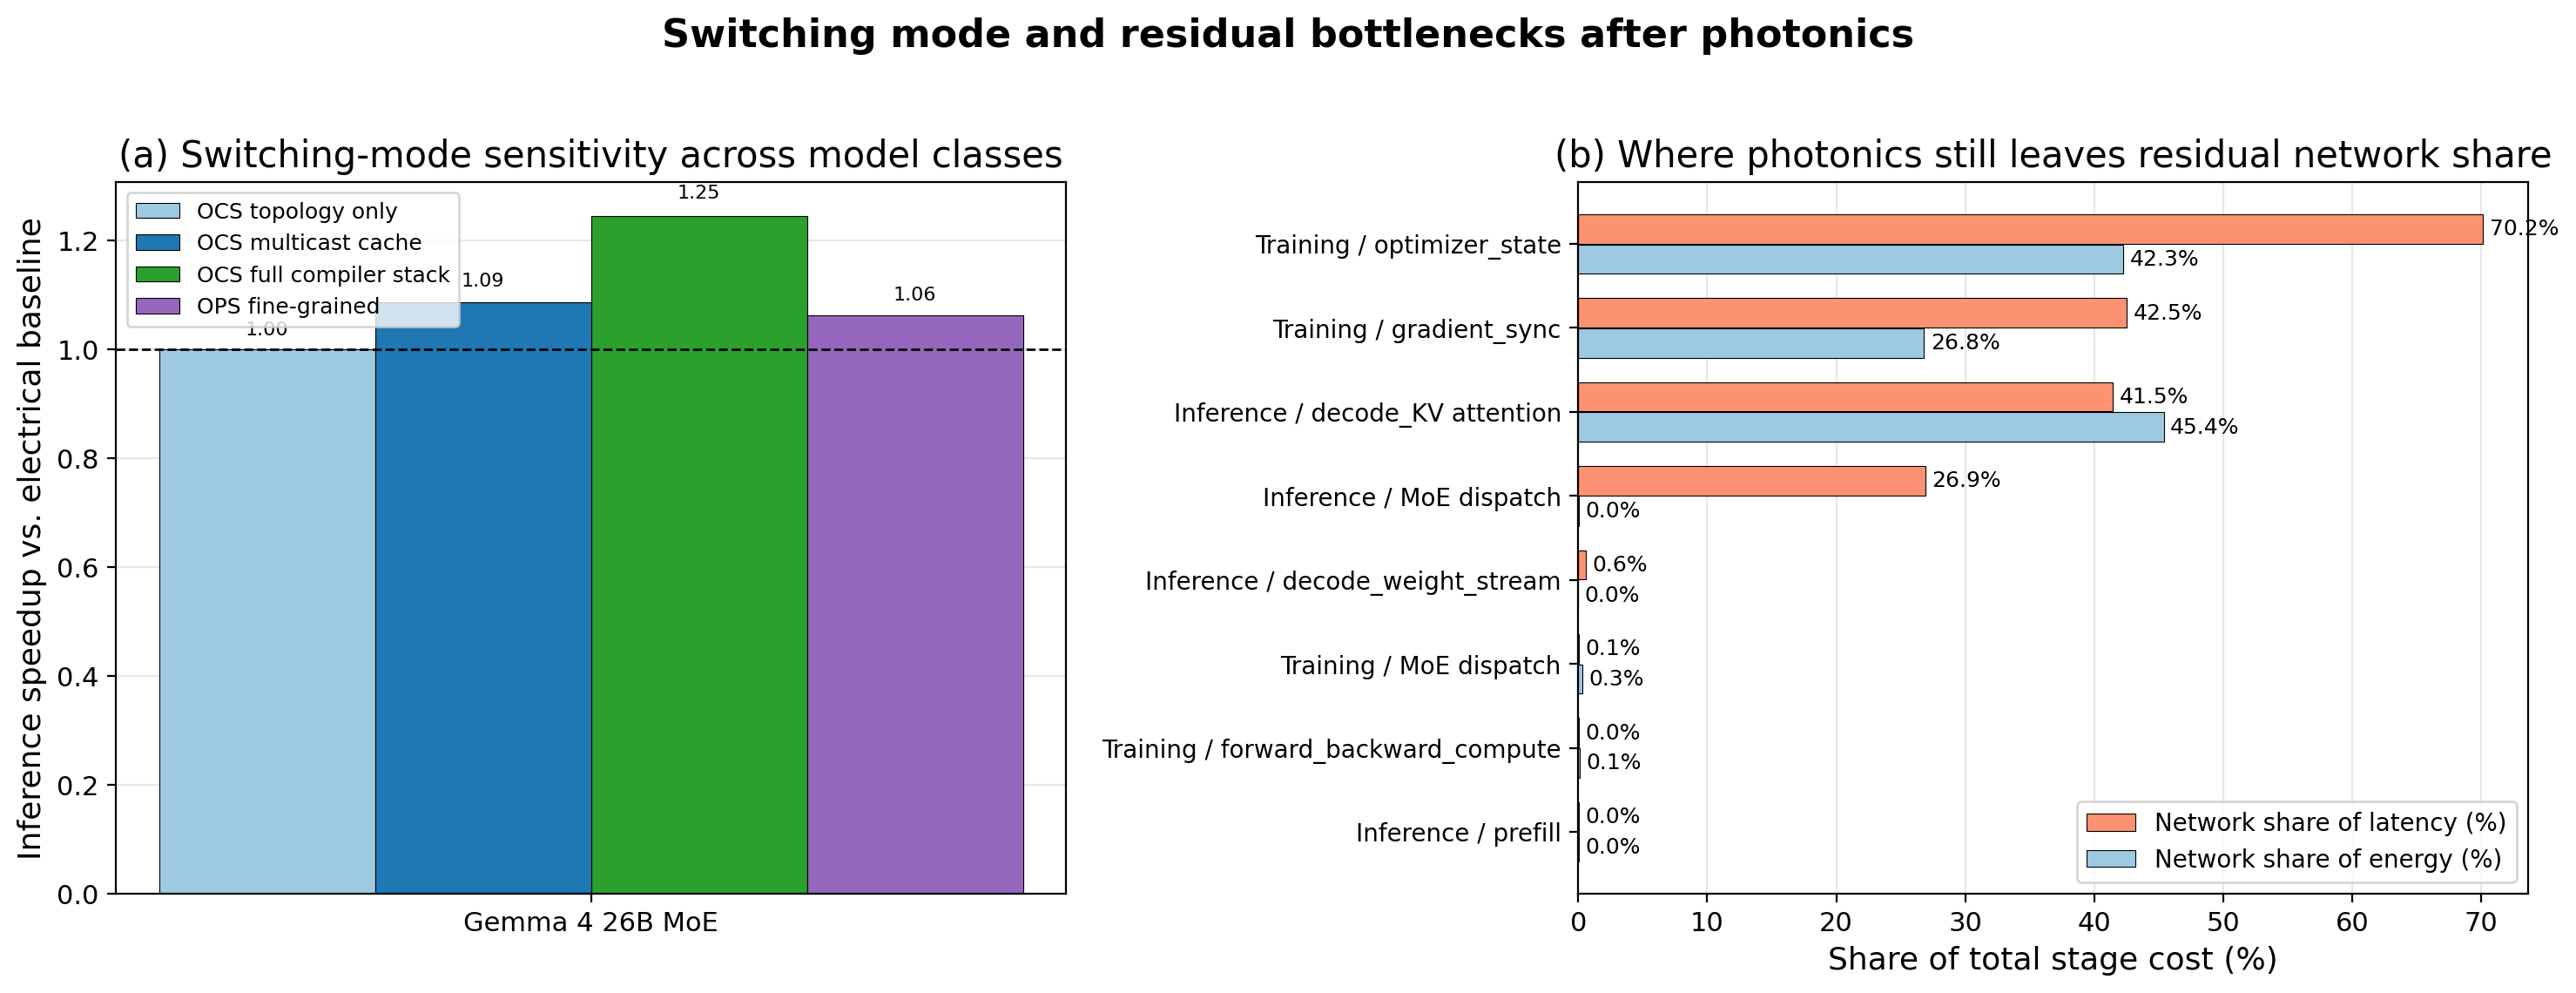
\includegraphics[width=\linewidth,height=0.78\textheight,keepaspectratio]{06_switching_and_limits.png}
\end{frame}

\begin{frame}{Reading Result 6}
  \begin{tightitemize}
    \item Topology alone, with no compiler change, brings the system to roughly parity with the electrical baseline. Layering multicast cache fill on top adds a small but measurable lift.
    \item Running the full compiler stack with multicast and remote pooled HBM is what moves the inference speedup into the $1.06\times$ to $1.25\times$ band relative to a topology-only switch baseline.
    \item Optical packet switching is included as a sensitivity point. It is not where most of the gain comes from---multicast and topology are.
    \item After photonics, the residual network share is concentrated in training optimizer-state and gradient-sync stages, which is where future work should focus.
  \end{tightitemize}
\end{frame}

\begin{frame}{Node-Count Scaling}
  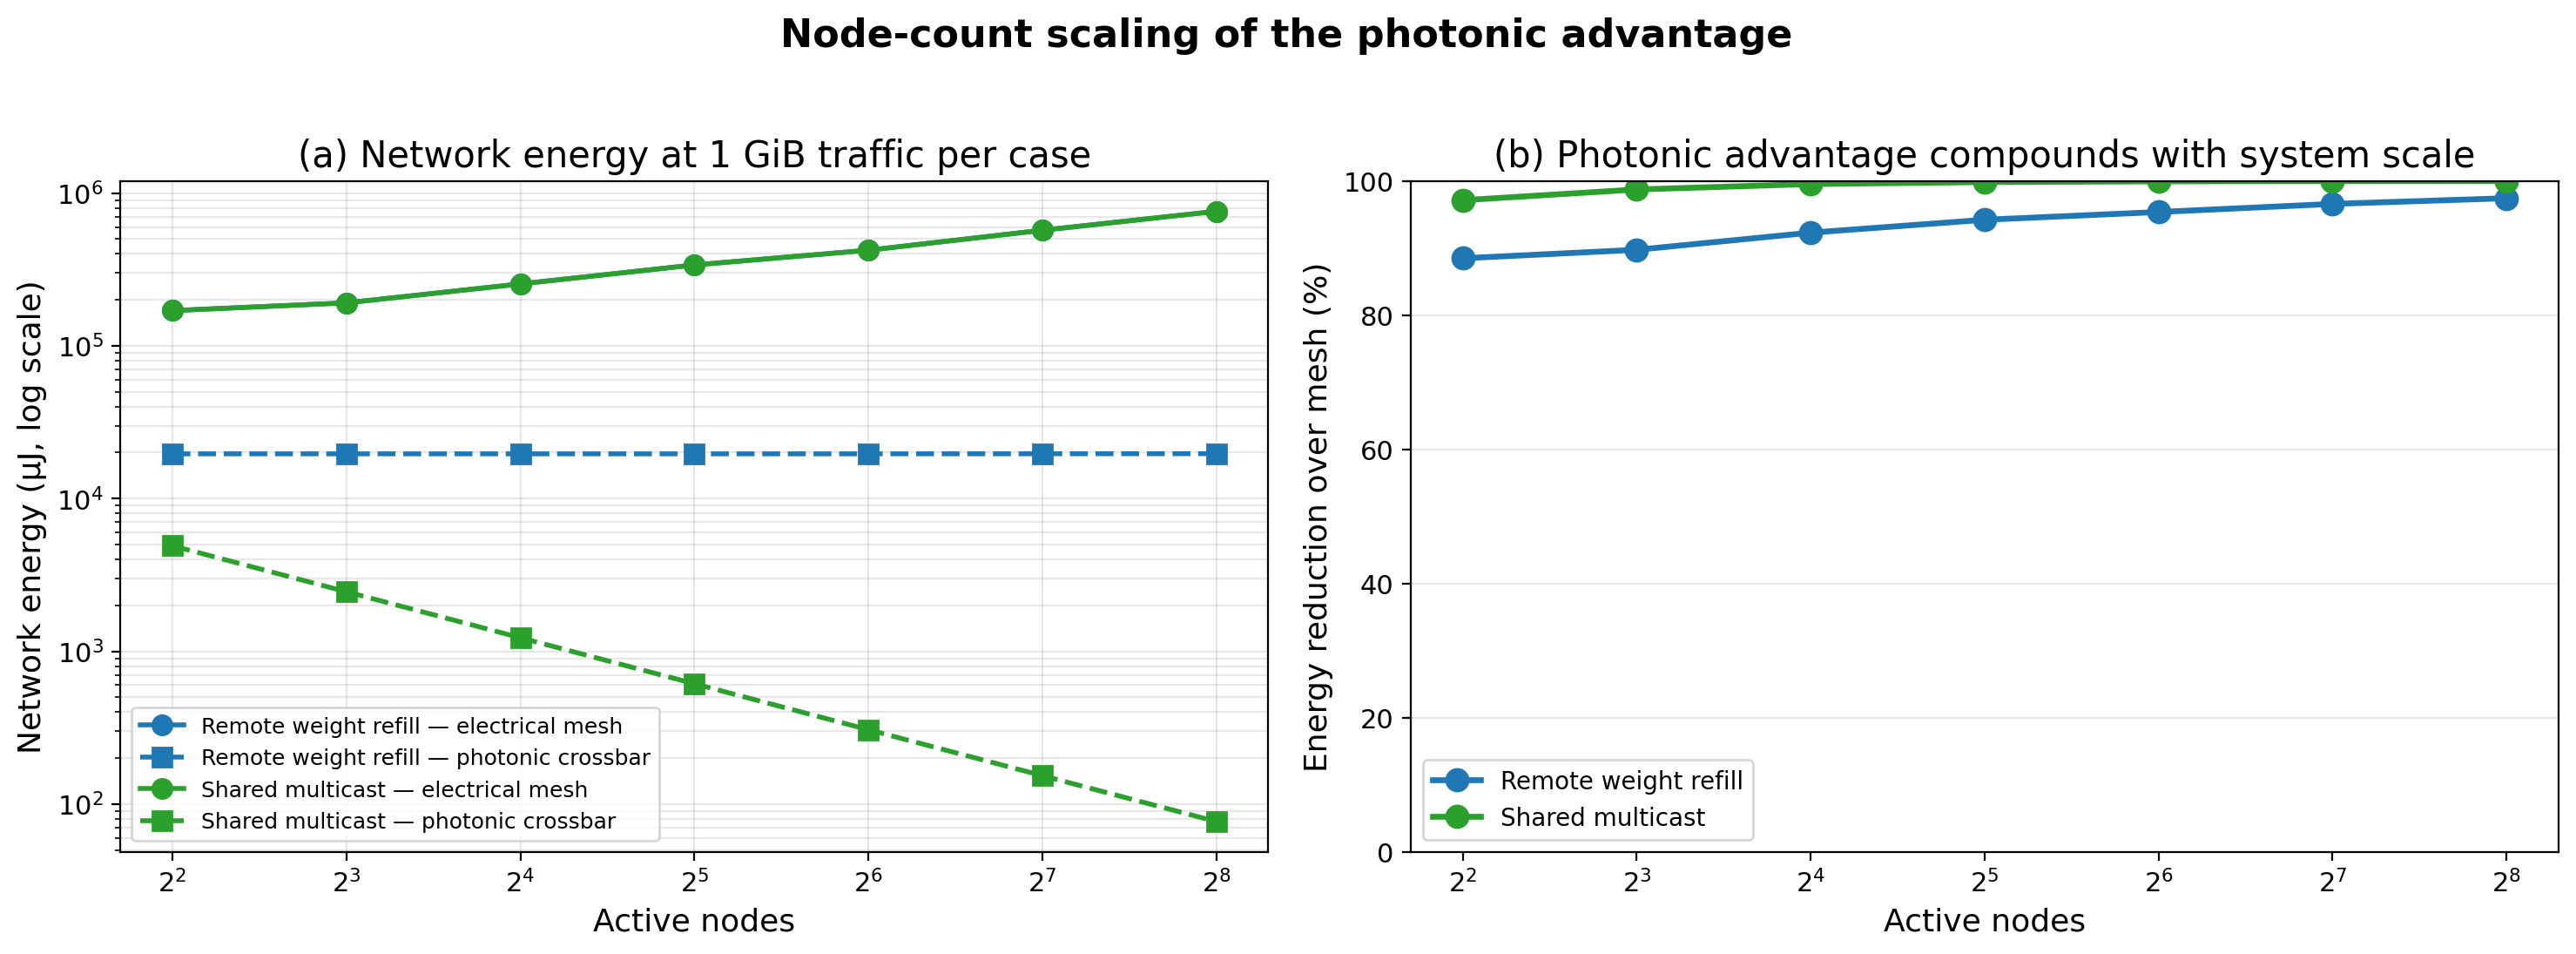
\includegraphics[width=\linewidth,height=0.78\textheight,keepaspectratio]{10_node_count_scaling.png}
\end{frame}

\begin{frame}{Headline Numbers}
  \scriptsize
  \begin{tabularx}{\linewidth}{lYY}
  \toprule
  Layer of the study & Result & Interpretation \\
  \midrule
  16-node cluster & 71.95\,\% energy, 97.57\,\% latency reduction & Logical-memory feedback loop visibly changes system metrics \\
  64-chip cube network & 99.93\,\% energy reduction & Multicast collapses repeated traffic \\
  64-chip cube mapping & $0/24$ inner mappings change & Local dataflow stays put \\
  Distributed schedule & $5/16$ choices change & Compiler-visible mapping is where the change lives \\
  Compiler strategy & 73.86\,\% best energy gain & Remote pooled-HBM and multicast cache fill can be optimal \\
  Pod inference (Gemma~4 MoE) & $42.4\times$ speedup, 94.05\,\% energy reduction & Decode, cache, and expert routing benefit most \\
  Pod training (Gemma~4 MoE) & $3.4\times$ speedup & Communication shrinks, then compute dominates \\
  \bottomrule
  \end{tabularx}
\end{frame}

\begin{frame}{What Worked, What Did Not}
  \begin{columns}[T,onlytextwidth]
    \begin{column}{0.48\textwidth}
      \begin{block}{Where photonics earned its place}
      \begin{tightitemize}
        \item Distance-aware physics at pod scale.
        \item Hardware multicast for shared state.
        \item Remote pooled-HBM streaming and multicast cache fill.
        \item Decode-heavy and mixture-of-experts inference.
      \end{tightitemize}
      \end{block}
    \end{column}
    \begin{column}{0.48\textwidth}
      \begin{block}{Where it did not}
      \begin{tightitemize}
        \item Local GEMM mappings did not move in the tested cases.
        \item Pure point-to-point unicast traffic gained the least.
        \item Training became compute-bound after collectives shrank.
        \item Detailed packet queueing, area and cost, thermal drift, and exact compiler code generation are out of scope.
      \end{tightitemize}
      \end{block}
    \end{column}
  \end{columns}
\end{frame}

\begin{frame}{Reproducibility and Validation}
  \begin{tightitemize}
    \item All quantitative results in these slides come from the same end-to-end study script, executed end-to-end, with both raw per-experiment data and a compact submission package committed to the repository.
    \item Every figure in this deck and in the report is regenerated from the same data tables. There are no hand-edited plots.
    \item A regression suite enforces the central physics (electrical-versus-photonic distance crossover), the multicast scaling law, the strong/weak scaling separation, the inner-mapping invariance claim, and the optical-switching sensitivity, so a future tweak to the catalog cannot silently invalidate the headline claims.
  \end{tightitemize}
\end{frame}

\begin{frame}{References}
  \scriptsize
  \begin{thebibliography}{9}
  \bibitem{tpu7x} Google Cloud, ``TPU7x (Ironwood),'' \url{https://docs.cloud.google.com/tpu/docs/tpu7x}
  \bibitem{m1000} Lightmatter, ``Passage M1000 EVK,'' \url{https://lightmatter.co/products/passage-m1000-evk/}
  \bibitem{evk100} Lightmatter, ``Passage EVK100,'' \url{https://lightmatter.co/products/passage-evk100/}
  \bibitem{passage} Lightmatter, ``Passage,'' \url{https://lightmatter.co/products/passage/}
  \bibitem{xla} PyTorch/XLA, ``SPMD User Guide,'' \url{https://docs.pytorch.org/xla/master/spmd.html}
  \bibitem{tcm} M. Gilbert, T. Andrulis, V. Sze, and J. Emer, ``The Turbo-Charged Mapper,'' arXiv:2602.15172, 2026.
  \end{thebibliography}
\end{frame}

\begin{frame}{Takeaway}
  \begin{block}{Final answer}
  Photonic interconnect is most valuable when the system above it can expose multicast, pooled memory, and flatter topologies to the compiler. The local accelerator mapping can stay where it is. The pod-level distributed schedule is what moves, and that movement is where the inference speedup lives.
  \end{block}
  \vspace{0.5em}
  \begin{center}
    {\Large Questions}
  \end{center}
\end{frame}

\end{document}
